\section{Durchführung}
\label{sec:Durchführung}
Die Grundplatte ist in Abb. \ref{fig:grundplatte} dargestellt.
Auf ihr befinden sich vier rechteckige Probestäbe aus Aluminium, (2x) Messing und Edelstahl.
Die Temperatur wird an zwei Stellen jedes Stabes gemessen.
Die Grundplatte wird an einer Spannungsquelle und an ein 8-fach Temperatur Array, das mit dem GLX Datenlogger verbunden ist angeschlossen.
Mit dem GLX Datenlogger können die Temperaturen gemessen und mit dem Xplorer GLX graphisch dargestellt und gespeichert werden.
Die Abstände zwischen den beiden Thermoelementen auf den jeweiligen Stäben müssen gemessen werden.
\begin{figure}
    \centering
    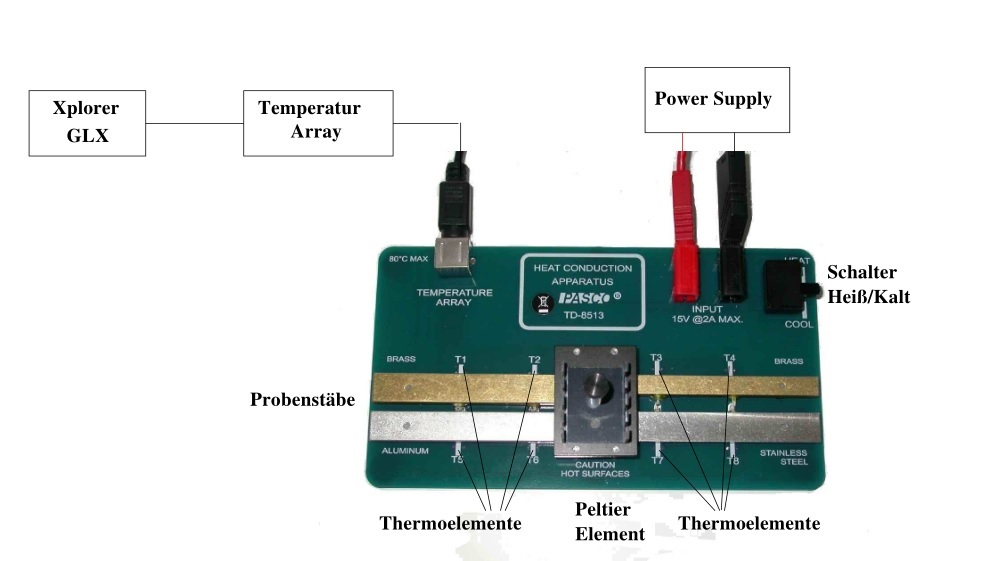
\includegraphics[width=0.75\textwidth]{content/data/glx.jpg}
    \caption{Die Grundplatte mit vier Probestäben und acht Thermoelementen. \cite[3]{anleitung}}
    \label{fig:grundplatte}
\end{figure}

\subsection{Statische Methode}
Die Spannungsquelle wird auf $U_\text{p} = \SI{5}{\volt}$ (bei maximalem Strom $I$) eingestellt und der Schalter auf "HEAT" gestellt.
Gleichzeitig wird die Messung für alle 8 Thermoelemente am Xplorer GLX mit der Abtastrate $\Delta t_\text{GLX} = \SI{5}{\second}$ gestartet.
Dabei ist darauf zu achten, dass die Wärmeisolierung auf den Stäben liegt.
Die Messung wird beendet, wenn die Temperatur des Thermoelements T7 $\SI{45}{\celsius}$ erreicht.
Im Anschluss wird der Schalter auf "COOL" gestellt, um die Stäbe zu kühlen.

\subsection{Dynamische Methode}
Die dynamische Methode wird auch als Angström-Messverfahren bezeichnet.
Der Probestab wird periodisch erhitzt.
Dadurch breitet sich eine Temperaturwelle mit einer bestimmten Ausbreitungsgeschwindigkeit aus, aus welcher die Wärmeleitfähigkeit bestimmt werden kann.
\\
Die Temperatur der Stäbe sollte nun unter $\SI{30}{\celsius}$ sein.
Die Abtastrate wird bei dieser Methode auf $\Delta t_\text{GLX}=\SI{1}{\second}$ gesetzt und die Spannungsquelle auf $U_\text{p} = \SI{8}{\volt}$ (bei maximalem Strom) eingestellt.
\\
Zuerst soll die Messung mit einer Periodendauer von \SI{80}{\second} durchgeführt werden.
Also wird die Messung gestartet, der Schalter auf "HEAT" gestellt und nach $\SI{40}{\second}$ zurück auf "COOL".
Nach weiteren $\SI{40}{\second}$ ist die erste Periode um.
Es sollten mindestens 10 Perioden gemessen werden.
\\
Um den Temperaturverlauf für Edelstahl zu messen ist eine Periodendauer von $\SI{200}{\second}$ notwendig.
Die Messung wird wie zuvor durchgeführt und beendet, wenn eins der Thermoelemente $\SI{80}{\celsius}$ anzeigt.